%!TEX root = ../thesis.tex
%*******************************************************************************
%****************************** Second Chapter *********************************
%*******************************************************************************

\chapter{Estado del Arte}

\ifpdf
    \graphicspath{{Chapter2/Figs/Raster/}{Chapter2/Figs/PDF/}{Chapter2/Figs/}}
\else
    \graphicspath{{Chapter2/Figs/Vector/}{Chapter2/Figs/}}
\fi

\section{Términos relacionados con el estilo de conducción}

El concepto de "Estilo de conducción" no tiene una definición estándar que sea aceptada en todo el mundo. Al contrario, este concepto involucra una serie de factores que aumentan su complejidad y complican su definición. Debido a esto se usarán los conceptos definidos por \citeauthor{8002632} \cite{8002632}.

\begin{figure}[htbp!]
\centering
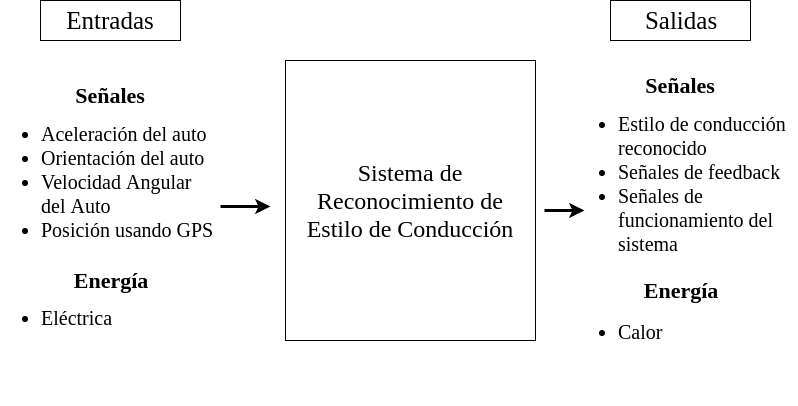
\includegraphics[width=0.8\textwidth]{Fig1}
\caption[Terminología estilo de conducción]{Terminología relacionada con el estilo de conducción \cite{8002632}}
\label{fig:2.1}
\end{figure}

Como se aprecia en la Fig~\ref{fig:2.1}, se entiende por un evento de conducción como las maniobras que se usan durante la acción de conducir, como por ejemplo: acelerar, desacelerar y girar.

De la misma manera, El patrón de conducción se define como el resultado de los eventos de conducción sujetos a condiciones de manejo, como el clima o el tipo de calzada. Este resultado se puede expresar como un perfil de velocidades. en el que están incluidos todos los datos que se pueden obtener partiendo de este perfil de velocidad, como por ejemplo: duración del viaje, velocidad promedio y demanda de potencia calculada.

La habilidad de conducción es la habilidad que posee el conductor para controlar el vehículo. Este concepto se usa para diferenciar entre un conductor experimentado o profesional de un conductor promedio.

El estilo de conducción es más complejo de definir debido a que para algunos autores involucra factores subjetivos como la actitud del conductor, el humor o el cansancio. Para \citeauthor{6957822} \cite{6957822}, el estilo de conducción  es la manera en la que la tarea de conducción es realizada. Esto se traduce en la forma en la que el conductor opera el vehículo (Pedal de aceleración, timón, freno, etc.). Esto se diferencia de el patrón de conducción tan solo porque no se asocia con un recorrido en especifico sino con un conductor.

También, se puede expresar el estilo de conducción en niveles de agresividad como \citeauthor{6294318} \cite{6294318}. Debido a que la agresividad en los eventos de conducción esta asociada con un mayor consumo de combustible y a menor seguridad vial, definitivamente juega un papel importante dentro del concepto de estilo de conducción. Esta es la forma en la que se definirá el estilo de conducción para esta tesis.

\section{Estado del arte según algoritmos usados}
Se procederá a mostrar las implementaciones e investigaciones desarrolladas en la actualidad clasificados según el tipo de algoritmo que se uso para la caracterización de el estilo de conducción

\subsection{Algoritmos basados en reglas}
Dentro de esta categoría se encuentran algoritmos de clasificación basados en reglas que comprenden el uso de lógica difusa, lógica difusa adaptativa y algoritmos de agrupamiento. Estos algoritmos se caracterizan por estar definidos por {\it umbrales predefinidos} y son el enfoque más sencillo para tratar de clasificar los estilos de conducción.

\citeauthor{6957822} \cite{6957822} desarrolló un sistema de reconocimiento de estilo de conducción online usando lógica difusa. Este sistema esta implementado usando {\it Matlab/Simulink}  y es paramétrico. Se puede configurar para ser usado en distintos tipos de vehículos.
El sistema detecta la aceleración longitudinal, aceleración lateral, desaceleración, velocidad, brecha de tiempo y activación del sistema autónomo de velocidad crusero. Además determina a través de un Sistema de Navegación el tipo de calzada en el que se encuentra (Se distingue entre trocha, calles urbanas, carreteras pavimentadas y carreteras rurales). Esto lo realiza debido a que el tipo de calzada influencia en gran medida al estilo de conducción. Por ejemplo, en una trocha la mayoría de conductores manejarían a una velocidad suave para no dañar al vehículo, lo cuál no necesariamente quiere decir que el mismo conductor conduzca de esa manera en otro tipo de escenarios.
Usando Lógica Difusa se definieron 3 niveles de estilo de conducción: {\it Normal, Confortable y Deportivo}. Se probó el sistema en una simulación y se obtuvieron los siguientes resultados promedio (Fig.~\ref{fig:2.2}): 67.8\% de clasificaciones correctas y solo 2\% de clasificaciones incorrectas (El otro 30.2\% pertenece a clasificaciones "Diferentes" que dan una clasificación contigua de estilo de manejo, por ejemplo cuando la clasificación real es {\it Normal} pero el sistema arroja como resultado {\it Confortable}, en cambio las clasificaciones incorrectas dan un resultado no contiguo al real)

\begin{figure}[htbp!]
\centering
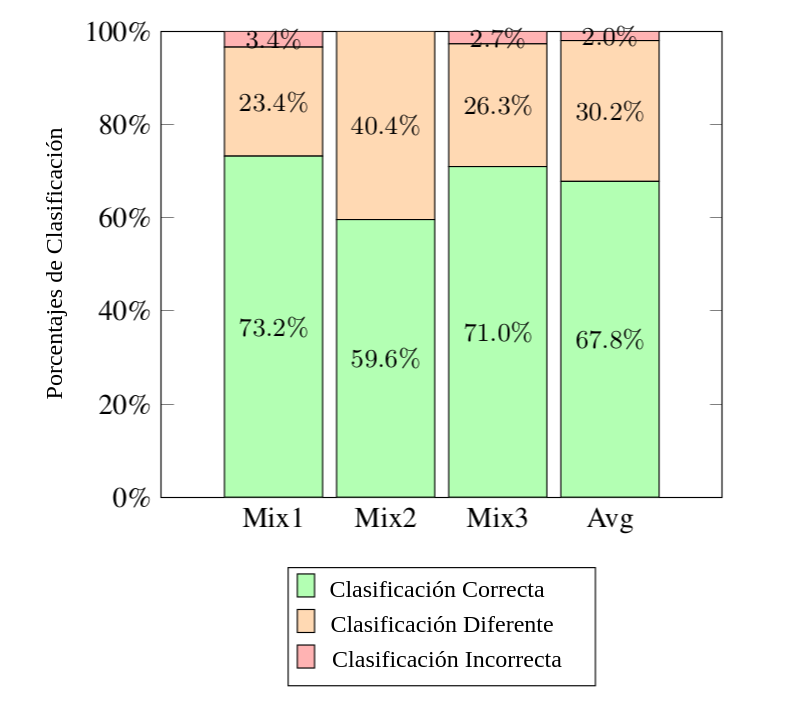
\includegraphics[width=0.8\textwidth]{Fig2}
\caption[Resultados del sistema de reconocimiento de estilo de conducción]{Resultados del sistema de reconocimiento de estilo de conducción en \cite{6957822}}
\label{fig:2.2}
\end{figure}

Usar lógica difusa no es la única manera de clasificar estilos de conducción. \citeauthor{4938719} \cite{4938719} presentó un método de clasificación basado en el análisis del perfil de la sobreaceleración (la derivada de la aceleración respecto al tiempo). En su investigación define al estilo de manejo como un comportamiento dinámico, Un conductor puede manejar de forma calmada por un momento y de forma agresiva en otro momento. Por este motivo, el método de clasificación que propone predice el estilo de conducción del usuario en tiempo real.
El algoritmo funciona de la siguiente manera:
\begin{enumerate}
    \itemsep0em
    \item Calcula el perfil de sobreaceleración durante una ventana de tiempo predefinido.
    \item Calcula la desviación estándar de la sobreaceleración durante toda la ventana de tiempo.
    \item Detecta el tipo de calzada actual y el nivel de congestión de tráfico usando el algoritmo propuesto en \cite{Highway_cap_manual}.
    \item Calcula la proporción de sobreaceleración dividiendo la desviación estándar con un valor promedio que depende de el tipo de calzada y el nivel de tráfico actuales.
    \item Dependiendo del resultado de la división realizada el conductor puede ser clasificado como {\it Calmado, Normal} o {\it Agresivo} usando reglas con umbrales predefinidos.
\end{enumerate}
\begin{figure}[htbp!]
\centering
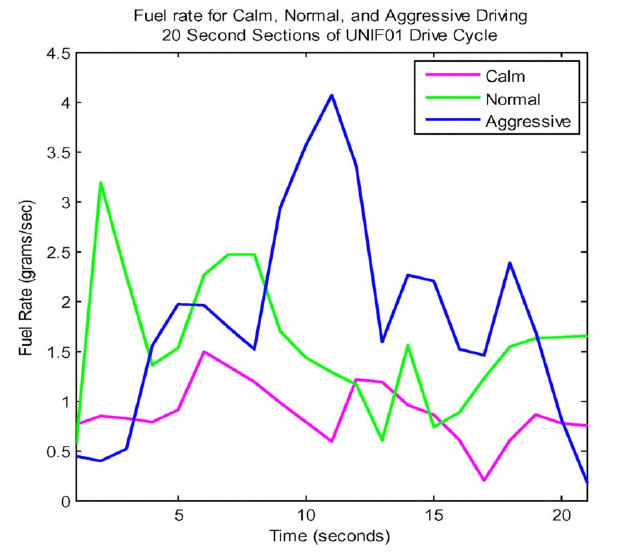
\includegraphics[width=0.75\textwidth]{Fig3}
\caption[Tasa de consumo de combustible según diferentes estilos de conducción]{Tasa de consumo de combustible según diferentes estilos de conducción \cite{4938719}.}
\label{fig:2.3}
\end{figure}
Este resultado dependerá mucho de la duración definida para la ventana de tiempo. Se recomendó usar una ventana de duración de 6 a 9 segundos para detectar los cambios de estilo de conducción oportunamente.

Se realizó también una comparación entre los 3 diferentes estilos de conducción con respecto a la tasa de consumo de combustible. Como se puede apreciar en la Fig.~\ref{fig:2.3}, los conductores clasificados como calmados están asociados a un menor consumo de combustible, mientras que los agresivos a un mayor consumo de combustible.

%para optimizar el uso de combustible. Por ejemplo en un vehículo híbrido, si el sistema predice que el conductor manejará de una manera agresiva, el sistema usará más potencia del motor eléctrico que del de combustión para así ayudar al ahorro de combustible.

Se ha presentado dos algoritmos basados en reglas que usan tanto múltiples variables \cite{6957822} como una sola \cite{4938719} para predecir el estilo de conducción del usuario. Sin embargo, los resultados de estos sistemas dependen en gran medida del valor de los umbrales escogidos para realizar la clasificación.

\subsection{Algoritmos basados en datos}
Cuando se tiene una cantidad muy grande de datos, es difícil analizarlos para obtener las reglas que guíen al algoritmo. Es entonces cuando los algoritmos basados en datos entran en acción. Estos algoritmos, en comparación con los basados en reglas, pueden manejar una mayor cantidad de datos y deducir umbrales consistentes con estos datos sin que estos dependan de un experto en el tema. A continuación se presentarán los distintos tipos de algoritmos basados en datos y su uso en el reconocimiento de estilos de conducción.

%********* Reinicia la cuenta de los \subsubsection y coloca el formato A,B,..****************************
\counterwithout{subsubsection}{subsection}
\renewcommand{\thesubsubsection}{\Alph{subsubsection}}
\preto{\subsection}{\setcounter{subsubsection}{0}}
%********************************************************************************************************

\subsubsection{Algoritmos de aprendizaje de máquinas no supervisados}
Los algoritmos no supervisados no necesitan que los datos obtenidos por medio de los sensores en la actividad de conducción estén etiquetados. Es decir, si se registra los datos de un ciclo de conducción para un conductor, este registro no necesita estar asociado con el estilo de conducción que mantuvo este conductor. Esta clase de algoritmos busca patrones en los datos y los segrega teniendo en cuenta sus similitudes y diferencias en diferentes grupos sin etiquetar.

\citeauthor{constantinescu} \cite{constantinescu} propuso el análisis de el estilo de conducción por medio de dos algoritmos: Hierarchical Cluster Analysis (HCA) y Principal Component Analysis (PCA).

HCA es un algoritmo de {\it machine learning} que trata de categorizar a cada individuo en grupos con características similares. Es muy útil cuando no se conoce con exactitud el número de grupos. Por medio de un análisis estadístico trata de minimizar la varianza dentro de cada grupo y a la vez aumentarla entre diferentes grupos. En este caso, el algoritmo de agrupamiento jerárquico consiste en empezar con grupos consistentes de un solo miembro y consecutivamente ir combinando los dos grupos más cercanos, hasta solo tener un grupo.

PCA es un método estadístico que usa una trasformación para convertir un posible conjunto de variables relacionadas entre si en otro conjunto menor de variables linealmente independientes, en las que la varianza sea maximizada.

Para este caso en particular se trabajo con dispositivo GPS que se encargaba de medir la velocidad y aceleración del vehículo monitorizado a una frecuencia de muestreo de \SI[mode=text]{1}{Hz}. De esta data se escogieron los siguientes parámetros:
\begin{enumerate}
    \itemsep0em
    \item Velocidad por encima de los \SI[mode=text]{60}{Km/h}.
    \item Velocidad promedio.
    \item Desviación estándar de la velocidad.
    \item Desviación estándar de la aceleración.
    \item Promedio de la aceleración positiva.
    \item Desviación estándar de la aceleración positiva.
    \item Promedio de la aceleración negativa o frenado.
    \item Desviación estándar del frenado.
    \item Trabajo mecánico, que se calculó sumando toda la energía cinética positiva requerida para aumentar la velocidad del vehículo.
\end{enumerate}

Luego del análisis realizado se encontraron 6 grupos o clusters y se describió cada uno de estos como se puede observar en el Tabla~\ref{diag:2.1} usando los 5 componentes principales resultantes al aplicar PCA.

\begin{table}[htbp!]
\centering
\caption[Descripción de los clusters obtenidos]{Descripción de los clusters obtenidos en \cite{constantinescu}.}
\begin{tabular}{crrrr}
\toprule
\multicolumn{1}{l}{\textbf{Cluster}} & \multicolumn{1}{c}{\textbf{Agresividad}} & \multicolumn{1}{c}{\textbf{Velocidad}} & \multicolumn{1}{c}{\textbf{Aceleración}} & \multicolumn{1}{c}{\textbf{Frenado}} \\ \midrule
1 & Moderadamente baja & Baja-Moderada & Moderada & Suave-Moderado \\
2 & Muy baja & Baja-Moderada & Baja-Moderada & Suave-Moderado \\
3 & Moderadamente alta & Moderada & Moderada & Repentino \\
4 & Neutral & Moderada & Alta & Moderado \\
5 & Neutral & Moderada-Alta & Baja-Moderada & Moderado-Repentino \\
6 & Alta & Alta & Alta & Repentino \\ \bottomrule
\end{tabular}
\label{diag:2.1}
\end{table}

Los algoritmos no supervisados tienen una gran ventaja, no se necesitan conocer las etiquetas de clasificación {\it a priori}. Esto significa que la definición de etiquetas no limita o influencia de alguna manera a los resultados obtenidos, ya que los grupos o clusters formados dependen solo de los datos usados. Sin embargo, luego de hallar los grupos se necesita realizar un análisis para determinar su naturaleza.

\subsubsection{Algoritmos de aprendizaje de máquinas supervisados}

Los algoritmos supervisados, a diferencia de los no supervisados, necesitan tener un conoci\-mien\-to previo de los datos que se tienen. Es decir, cada uno de los datos recolectados deben estar asociados a una etiqueta o clase ya predefinida.

Uno de los algoritmos más utilizados es el de K-Nearest Neighbors (k-NN), que se utilizó junto a Dynamic Time Warping (DTW) en el sistema de reconocimiento propuesto por \citeauthor{6083078} \cite{6083078}. El objetivo de este sistema es reconocer maniobras agresivas para dar un feedback al conductor y monitorizarlo, mejorando así la seguridad vial. Para lograrlo usaron los sensores presentes en un smartphone (acelerómetro, giroscopio, GPS y cámara frontal). Este sistema trabaja grabando la información de todos los sensores durante 5 minutos, luego analiza si ha ocurrido alguna maniobra potencialmente agresiva. Si una maniobra de este tipo ocurrió, conserva la información para un análisis posterior. En cambio, si no ocurrió ninguna maniobra de este tipo, borra la data para ahorrar espacio en disco.

Para la clasificación de cada maniobra detectada se usa Dynamic Time Warping (DTW), el cual es un algoritmo que es capaz de analizar la similaridad entre dos señales que no necesariamente tengan la misma duración y probablemente tengan un desfase. En la Fig.~\ref{fig:2.4} se puede observar una comparación entre una comparación de una distancia Euclidiana y otra usando DTW en dos señales muy parecidas en forma pero que no se encuentran en fase.


\begin{figure}[htbp!]
\centering
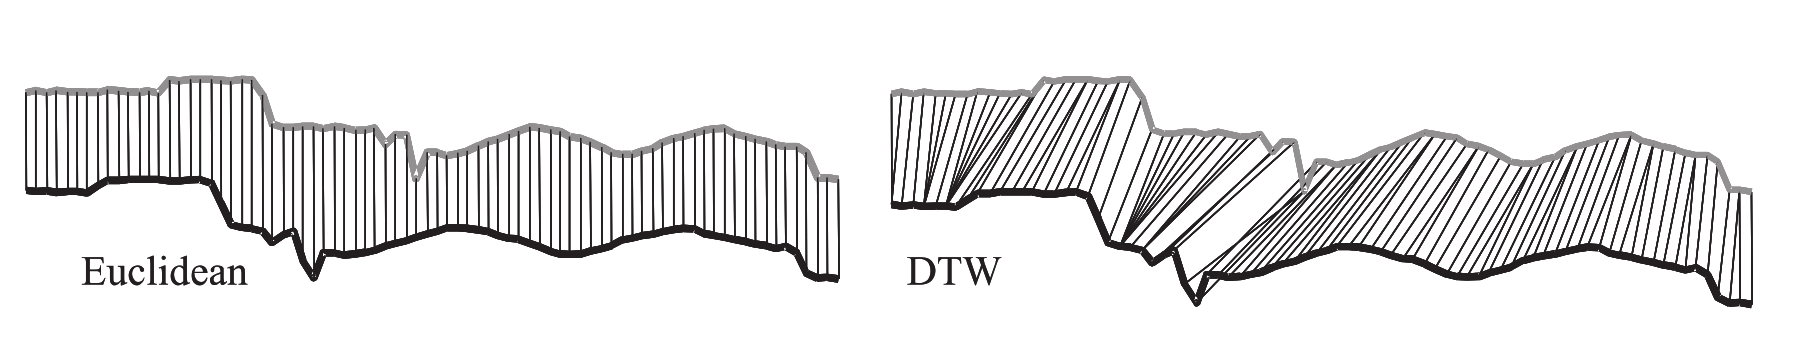
\includegraphics[width=0.95\textwidth]{Fig4}
\caption[Comparación de señales usando distancia Euclidiana y DTW]{Comparación de señales usando distancia Euclidiana y DTW \cite{Keogh2005}.}
\label{fig:2.4}
\end{figure}

El algoritmo consiste en crear una matriz de deformación $n \times m$, siendo $n$ y $m$ los números de puntos en cada señal. Esta matriz se llena calculando distancias entre cada punto, sin importar si se encuentran en el mismo instante temporal. Luego se dibuja el camino con la distancia más corta que une el inicio de las señales con el final de estas Fig.~\ref{fig:2.5} {\bf (B)}. La suma de distancias en este camino se define como la distancia entre las dos señales analizadas y se puede usar para comparar la similitud y clasificar señales usando modelos. Información detallada sobre este algoritmo se puede encontrar en \cite{Keogh2005}.
\begin{figure}[htpb!]
\centering
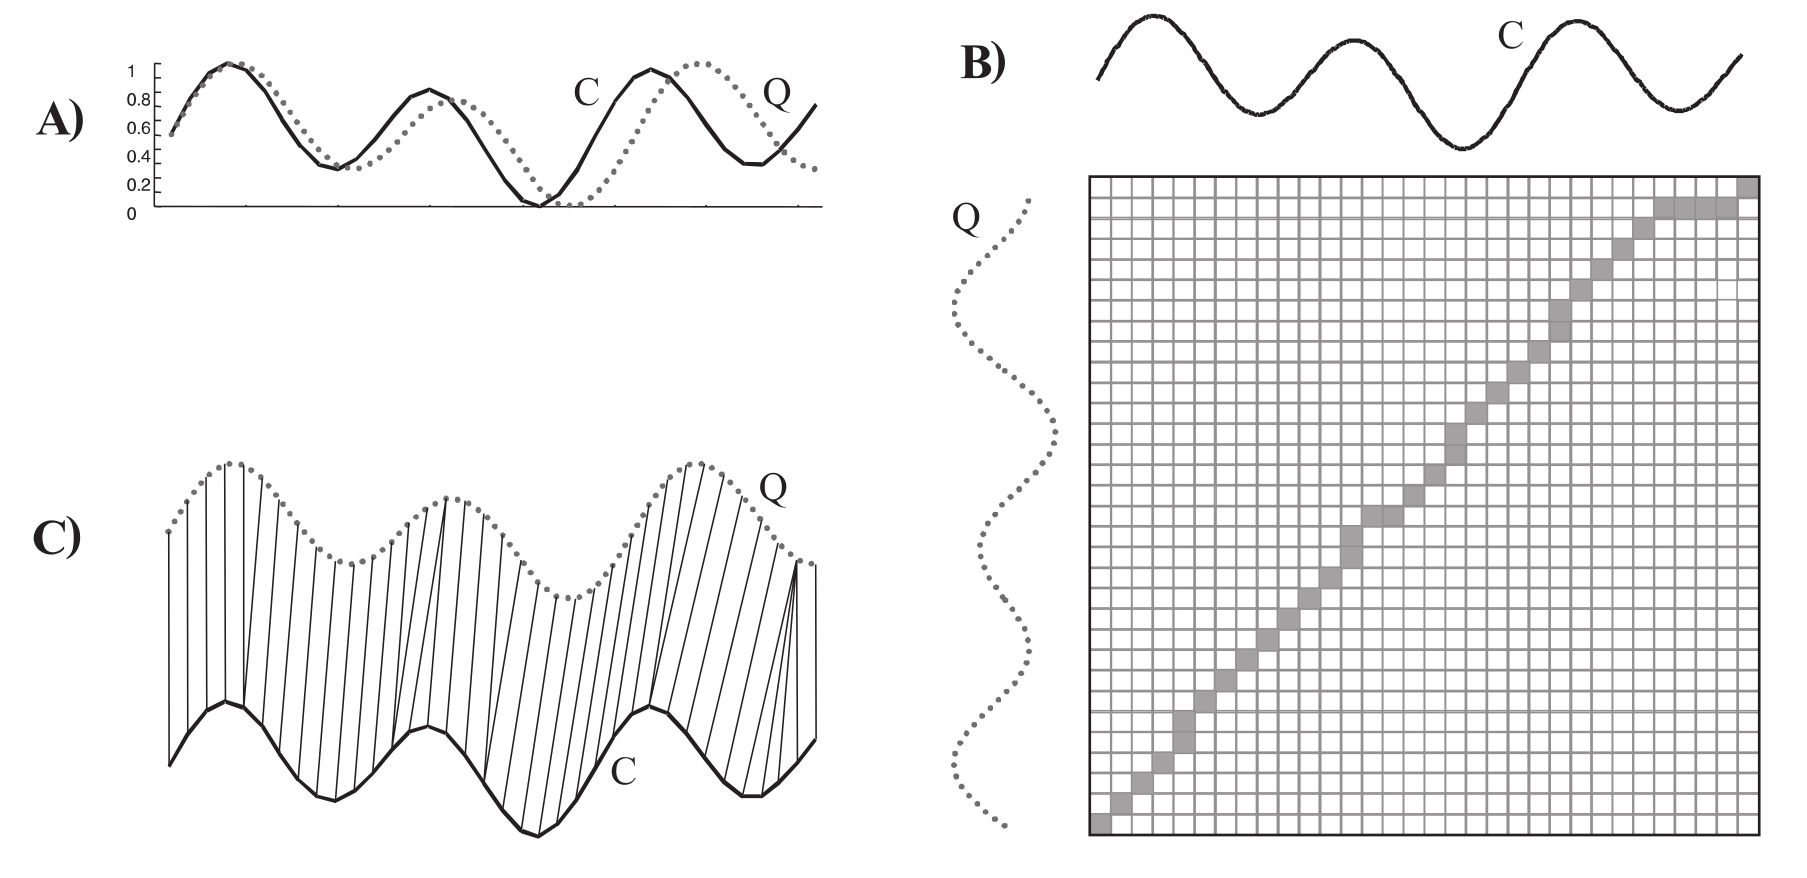
\includegraphics[width=0.85\textwidth]{Fig5}
\caption[Algoritmo de {\it Dynamic Time Warping}]{{\bf A)} Dos señales con forma muy similar pero desfasadas. {\bf B)} Matriz de deformación usada para encontrar el camino de deformación. {\bf C)} El resultado del alineamiento y deformación usando DTW. \cite{Keogh2005}.}
\label{fig:2.5}
\end{figure}

Para poder usar DTW se necesitó contar con señales modelo para cada tipo de maniobra a detectar. Se tuvo un total de 120 señales modelo en total, cada una asociada con una maniobra específica.  Usando DTW se puede obtener una medida de distancia entre las señales a clasificar y las señales modelo. Luego se aplicó K-Nearest Neighbors (k-NN) para clasificar cada señal. Lo que hace k-NN es tener en guardadas las señales modelos y al momento de clasificar una nueva señal calcula la distancia con las señales modelos, selecciona las $k$ distancias menores y dependiendo de la clase que tenga más señales cercanas, esta nueva señal es clasificada.

Para realizar la clasificación de señales solo se utilizó los datos de $g_x$, $a_y$ y $e_x$ (giroscopio en $x$, aceleración en $y$ y ángulo de rotación de Euler en $x$ respectivamente). Se puede observar en el Tabla.~\ref{diag:2.2} los porcentajes de reconocimiento exitoso por cada maniobra.

% Please add the following required packages to your document preamble:
% \usepackage{booktabs}
\begin{table}[htbp!]
\centering
\caption[Porcentaje de reconocimiento de maniobras de conducción]{Porcentaje de reconocimiento exitoso de maniobras de conducción \cite{6083078}.}
\begin{tabular}{@{}lc@{}}
\toprule
Maniobra & \multicolumn{1}{l}{\begin{tabular}[c]{@{}l@{}}Porcentaje de reconocimiento exitoso (\%)\end{tabular}} \\ \midrule
Giro a la derecha (\ang{90}) & 92 \\
Giro a la izquierda (\ang{90}) & 83 \\
Vuelta en U (\ang{180}) & 77 \\
Giro a la derecha agresivo & 100 \\
Giro a la izquierda agresivo & 100 \\
Vuelta en U agresiva & 100 \\
Cambio de carril agresivo (derecha) & 100 \\
Cambio de carril agresivo (izquierda) & 83 \\ \bottomrule
\end{tabular}
\label{diag:2.2}
\end{table}

Otro algoritmo aplicado usualmente al reconocimiento de estilos de manejo es el uso de {\it Redes Neuronales}. \citeauthor{7727682} \cite{7727682} utilizó redes neuronales para clasificar estilos de manejo y {\it Algoritmos Genéticos} para optimizar estas redes e incluso elegir los parámetros de entrada. El sistema que propuso se enfocaba en obtener un clasificador que pueda ser utilizado por un sistema embebido de potencia baja. Por lo cuál utilizo un tipo de red neuronal llamado {\it Extreme Learning Machines}. Este tipo de red neuronal, como se observa en la Fig.~\ref{fig:2.6}, se caracteriza por tener tan solo una capa oculta entre las entradas y las salidas. Además se eligen los pesos entre las entradas y la única capa oculta de manera aleatoria y nunca se actualizan. Esta red neuronal solo aprende los pesos entre la capa oculta y las salidas en una sola iteración. Por esta razón este tipo de red resulta siendo muy ligero y de entrenamiento muy veloz.

\begin{figure}[htpb!]
\centering
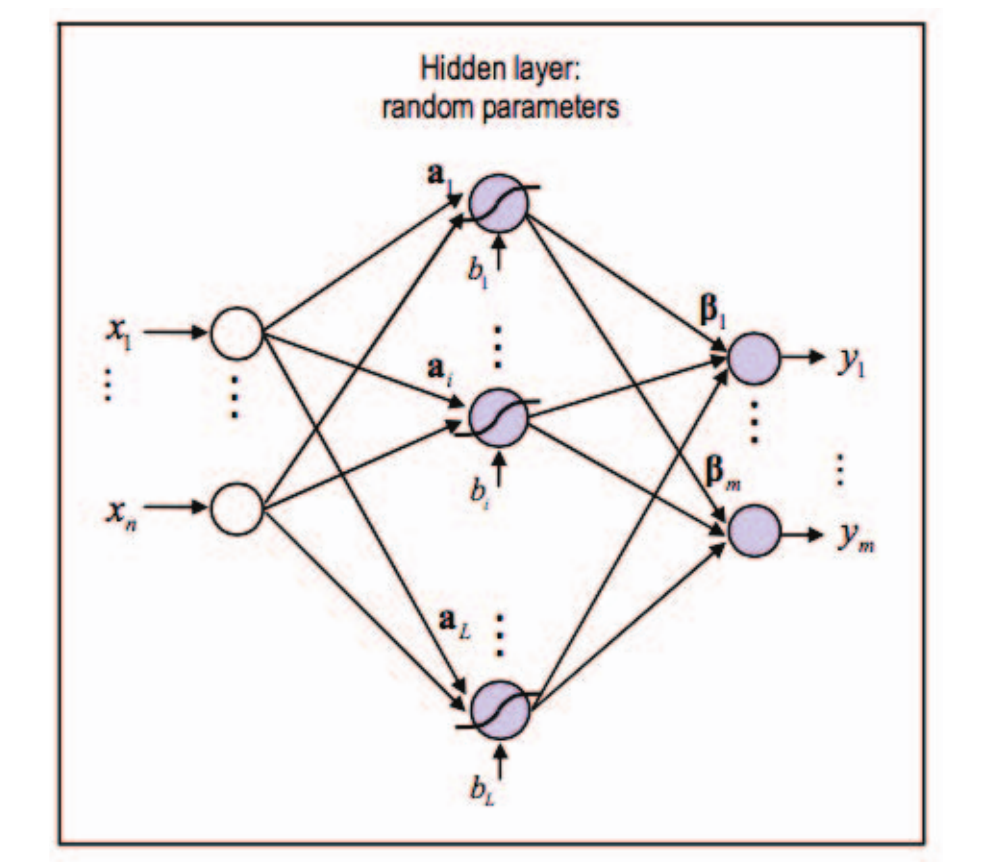
\includegraphics[width=0.8\textwidth]{Fig6}
\caption[Topología de una Red Neuronal usada para Extreme Learning Machines]{Topología de una Red Neuronal usada para Extreme Learning Machines \cite{7727682}.}
\label{fig:2.6}
\end{figure}

\citeauthor{7727682} recolectó un conjunto de 21 variables de 11 conductores, pero no utilizó toda la información. En lugar de eso utilizó un algoritmo genético llamado {\it Non-Dominated Sorting Genetic Algorithm}. Este tipo de algoritmo genético realiza una optimización multiobjetivo. Lo cual significa que trata de optimizar más de una variable a la vez. En este caso se trata de minimizar 3 variables: el número de atributos de entrada para la red neuronal, el número de neuronas en la capa oculta y la tasa de error resultante de la red neuronal entrenada.

Normalmente no existe una solución que permita minimizar las 3 variables a la vez. Debido a esto, lo que se busca en realidad se conoce como {\it Soluciones Óptimas de Pareto}. Este término hace referencia a las soluciones en las que no se puede optimizar ninguna variable sin degradar a otra. Este tipo de algoritmos genéticos contiene el concepto de Soluciones óptimas de Pareto como función de fitness, de tal manera que permite optimizar las 3 variables antes mencionadas.

Finalmente, se escoge una solución que tiene un 90.1\% de tasa de reconocimiento, 8 entradas para la red neuronal y 16 neuronas en la capa oculta.

\subsubsection{Algoritmos que combinan los enfoques supervisados y no supervisados}

Los algoritmos supervisados y no supervisados aparecen como dos categorías totalmente separadas. Sin embargo, esto no significa que no se puedan usar juntos y combinar para mejorar sus ventajas o reducir sus desventajas.

\citeauthor{6629603} \cite{6629603} propuso un sistema
que utiliza los sensores inerciales embebidos en un auto para identificar posibles maniobras inseguras y proporcionar un adecuado feedback hacia el conductor. Además también propone caracterizar y diferenciar conductores solo usando datos de los sensores inerciales, para poder diferenciar cuando dos personas distintas utilizan un mismo vehículo. Para lograr su objetivo primero analiza la información de los sensores para determinar un conjunto básico de maniobras: frenado, aceleración y giro.


Se utiliza el algoritmo de aprendizaje no supervisado {\it K-means Clustering} para identificar las maniobras. Este algoritmo consiste en generar $k$ semillas, de preferencia no aleatorias ya que la inicialización tiene una gran influencia en los clusters resultantes, que representarán la media o el centroide de cada cluster, luego por medio de la definición de una métrica de distancia (Euclidiana, citiblock, etc.) se asignan los datos al cluster del centroide más cercano. Luego de clasificar a todos los datos se vuelve a calcular el centroide de cada cluster (que muy probablemente cambiará de posición) y se repite los pasos hasta converger en una posición de centroides.


Al identificar las maniobras se usan dos fuentes de datos distintas: la primera cuenta con la inforamcion completa de los sensores, asi como también un análisis estadístico de estos (mínimo, máximo, media, varianza, etc.); en cambio, la segunda solo cuenta con el análisis estadístico. Y los resultados que se obtienen son muy similares. El desempeño de el clasificador no se reduce al no incluir los datos completos de los sensores, sino que puede usar tan solo sus datos estadísticos.

Luego se utiliza el algoritmo supervisado {\it Support Vector Machines} (SVM). Este algoritmo usa los datos con sus respectivas clases y trata de crear un hiperplano que separe todos los datos pertenecientes a una clase de la otra. Mientras este hiperplano tenga una mayor distancia con los miembos más cercanos de ambas clases, se tendrá un menor error de generalización. El encontrar este hiperplano que separe a las dos clases en la mayoría de los casos no es posible en el espacio definido por los atributos actuales de los datos. Debido a esto se mapean los datos en un espacio con más dimensiones para lograr encontrar este hiperplano de una manera más sencilla.

\section{Estado del arte según sensores usados}

Para usar los algoritmos mencionados anteriormente se han usado diferentes clases de sensores para medir distintas variables, ya sea directa o indirectamente. En el Tabla~\ref{diag:2.3} se puede apreciar los sensores utilizados en las investigaciones mencionadas.

\begin{table}[htpb!]
\centering
\caption{Resumen de sensores usados en las investigaciones mencionadas}
\begin{tabular}{@{}ll@{}}
\toprule
Sensores usados & Referencias \\ \midrule
Inertial Measurement Unit (IMU)& \cite{4938719}, \cite{7727682}, \cite{6629603} \\
Acelerómetros de bajo costo & \cite{6294318} \\
Smartphone & \cite{6083078} \\
GPS & \cite{constantinescu} \\
GPS e IMU & \cite{6957822} \\ \bottomrule
\end{tabular}
\label{diag:2.3}
\end{table}

\subsection{Acelerómetros de bajo costo}
Los acelerómetros nos permiten medir la aceleración longitudinal y lateral, que son las que nos permiten medir eventos de conducción como el frenado y la aceleración o los giros. Con un acelerómetro de 2 ejes como el usado en {6294318} es suficiente para medir estas dos aceleraciones.

Estos acelerómetros pueden costar desde \textdollar 2, como el MMA6910KQ \cite{acelerom} que consta de 3 ejes y puede tener un rango de $\pm 3.5$ o $\pm \SI{5.0}{g} $.

\subsection{Smartphone}
Los smartphones tienen cada vez más y más sensores que pueden ser usados para aplicaciones como las de la presente tesis. En \cite{6083078} se usó los sensores integrados en un Iphone 4 para realizar la tarea de reconociento de estilo de conducción. Estos sensores fueron la cámara trasera (solo para registro), el acelerómetro de 3 ejes, el giroscopio de 3 ejes y el GPS. \newpage

\subsection{Inertial Measurement Unit}
Esta clase de sensores se puede encontrar bajo un rango de precios muy amplio. Existen unidades por debajo de los \textdollar 10 como el MPU-6050 (Fig.~\ref{fig:2.7}) que cuenta con un giroscopio de 3 ejes y un acelerómetro de 3 ejes; y funciona a un voltaje de \SI[mode=text]{2.3}{V} a \SI[mode=text]{3.4}{V} \cite{invensense}

\begin{figure}[htpb!]
\centering
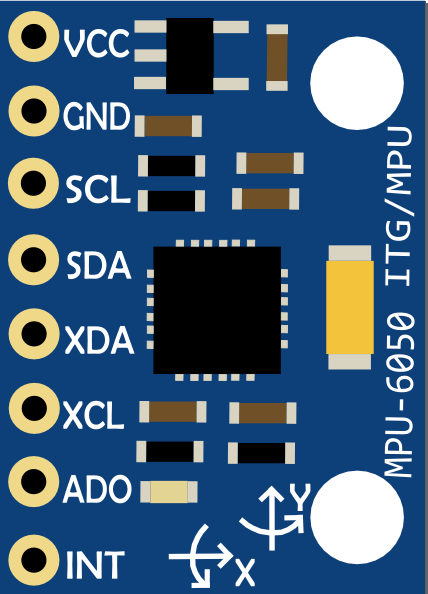
\includegraphics[width=0.3\textwidth]{Fig7}
\caption[MPU-5050 de Invensense]{MPU-6050 de Invensense \cite{invensense}.}
\label{fig:2.7}
\end{figure}

\subsection{GPS}
El GPS es muy usado también al reconocer estios de conducción ya que aporta información muy relevante al sistema, por ejemplo se puede usar la información del GPS para detectar el tipo de camino en el que se encuentra el auto en ese momento. Además se puede usar también para obtener la velocidad del auto, aunque es más usado en conjunto con un IMU para que al combinar la información de ambos sensores se usen algoritmos de {\it Sensor Fusion} para mejorar el resultado de las mediciones.

\section{Feedback}
Una de los elementos más importantes de los sistemas de reconocimiento de estilos de conducción antes mencionados son las señales de feedback que se le dan al conductor. Dependiendo de cuál sea el enfoque del reconocimiento de estilo de conducción (enfoque en ahorro de combustible o enfoque en agresividad de maniobras).

Hay 3 maneras principales de generar este feedback. De manera visual, háptica, audible o una combinación de estos. Cada una presenta ventajas y desventajas.

Para generar feedback de manera visual se pueden incluir Human Machine Interfaces (HMI), que básicamente son pantallas que permiten al conductor saber que estilo de conducción se encuentran ejerciendo en ese momento. Esto se podría lograr usando un un smartphone o una tablet también. La desventaja de usar feedback visual es el conductor ya procesa mucha información visual al llevar a cabo la tarea de conducir, por lo que agregar más información requiere que el conductor preste atención al dispositivo  y reduzca su atención en el camino. Esto podría presenta problemas de seguridad como se señala en \cite{benedetto2012}

En \cite{8207769} se usó una tablet como método de feedback para entregar {\it Tips de Conducción} al usuario. El sistema funcionaba de las siguiente manera: Reconocia el estilo de conducción actual del conductor y se usaba {\it Learning Path Planning} para poder llegar desde el estilo de conducción detectado a uno óptimo en el que se consuma menos combustible. Obtenido esto, se procedían a mostrar los tips de conducción al conductor usando la tablet. En este sistema se lograba incrementar la economía del combustible en un 6.25\%.

Para generar señales auditivas se puede utilizar un pequeño parlante que haga sonar una alarma cuando se registra un comportamiento no deseado del conductor (Estilo de conducción con alto consumo de combustible o muy agresivo). Este método

Por último, las señales hápticas han sido investigadas debido a que es el único canal de información por el cual los conductores no reciben mucha información de la tarea de conducir. Lo que quiere decir, que generaría menos distracciones que los otros tipos de feedback. En \cite{Hapticreview} se expone diferentes maneras de entregar esta señal (En el timón, el panel frontal del auto, el asiento , etc.).


